
\subsection{研究背景}

\subsubsection{Mesa3D顶点数组绘制模式实现原理}
从前面的立即模式实现原理我们可以看到顶点数据是一个个的搬运到VRAM上的buffer上的,当我们绘制拥有大量数据的图形时候,这样一点点的搬运就显得非常的缓慢了,当然我们可以尝试使用显示列表来对这些数据进行预编译,需要遍历这些顶点数据然后把数据传给GPU的显存。但是这些数据不一定是静态的,有可能在我们每次渲染的时候,我们需要对这些数据进行更改。这个时候就不适合使用显示列表了。

为了很好的解决这个问题。我们可以使用顶点数组,我们可以随时进行预编译或修改几何图形,然后一次性传输这些数据。顶点数组的绘制模式相对于立即模式极大的提高了绘制效率。使用顶点数组有3个基本的步骤:

\begin{itemize}
\item{} 激活(启用)最多可达8个数组,每个数组用于存储不同类型的数据: 顶点坐标,表面法线,颜色等等。
\item{} 把数据放入数组中。这些数组是通过它们的内存位置的地址(即指针)进行访问。
\item{} 用这些数据绘制几何图形。OpenGL通过指针从所有激活的数组中获取数据。
\end{itemize}

我们还是以svPerfGL的顶点数组模式测试项为研究对象来分析Mesa3D顶点数组的实现原理:

\begin{lstlisting}
glEnableClientState(GL_VERTEX_ARRAY);
glVertexPointer(3, GL_FLOAT, sizeof(float)*3, (const GLvoid *)tVerts);
glEnableClientState(GL_NORMAL_ARRAY);
glNormalPointer(GL_FLOAT, sizeof(float)*3, (const GLvoid *)tNorms);
glEnableClientState(GL_COLOR_ARRAY);
glColorPointer(3, GL_FLOAT, sizeof(float)*3, (const GLvoid *)tColors);

glDrawArrays(GL_TRIANGLES, 0, tNumVerts);
\end{lstlisting}

这里在介绍Mesa3D顶点数组实现原理之前先介绍一个重要的数据结构:
\begin{lstlisting}
struct pipe_vertex_buffer{
   ...
   struct pipe_resource *buffer; 
   const void *user_buffer;
};

struct pipe_vertex_buffer vertex_buffer[PIPE_MAX_ATTRIBS];
\end{lstlisting}
这里vertex\underline{ }buffer数组就是存放着各个属性数据数组的指针,当我们使用传统的立即模式时候,这些指针就指向着前面一节说到的VRAM上的buffer(struct pipe\underline{ }resource *buffer),而在我们使用顶点数组模式时候,这些指针就指向着我们用户准备的顶点数据数组(const void *user\underline{ }buffer)。所以在顶点数组模式下,在glVertexPointer()这类函数执行时候,Mesa3D会把用户指定的数组指针添加到对应vertex\underline{ }buffer[]数组里面的user\underline{ }buffer中。接着我们调用glDrawArrays()之类的函数进行顶点数组模式绘制时候,Mesa3D会执行u\underline{ }vbuf\underline{ }upload\underline{ }buffers函数将用户定义的顶点数组数据通过memcpy()函数从内存拷贝到显存中,然后像之前的立即模式一样向GPU发送绘制命令执行硬件渲染。

\begin{figure}[H] 
  \centering
  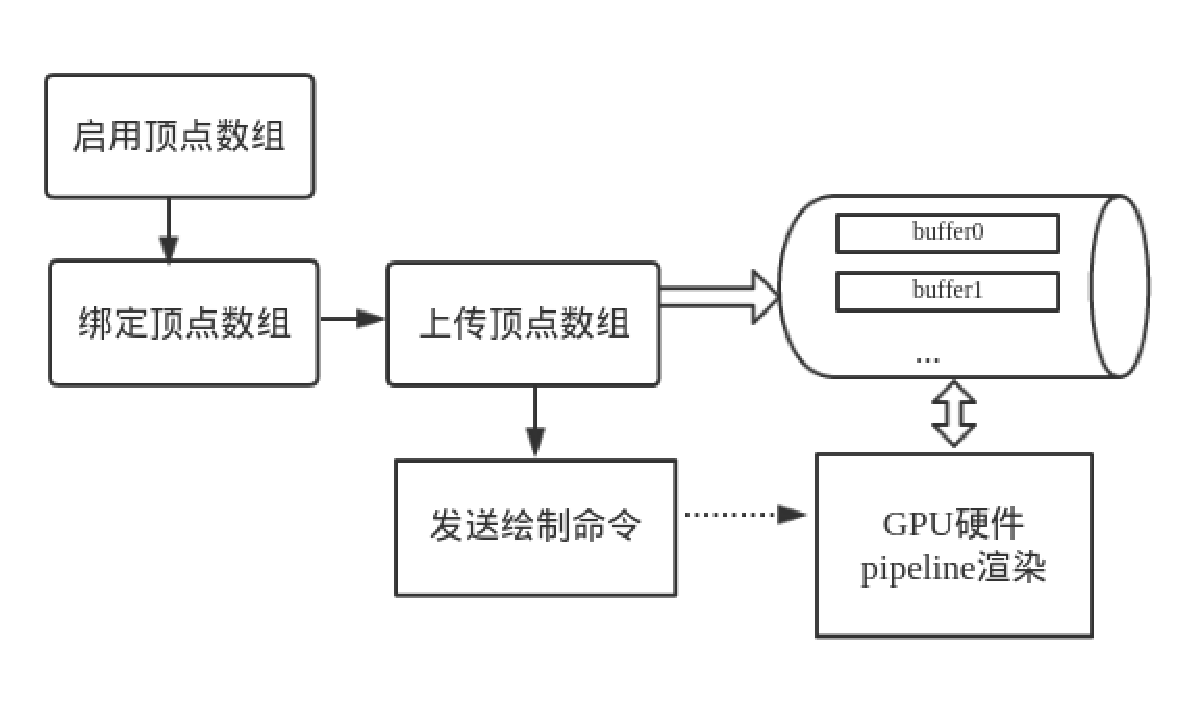
\includegraphics[width=12cm,height=8cm]{figures/chap03/vbo-flow}
  \caption{Mesa3D图形库顶点数组模式实现机制}
  \label{fig:vbo-flow}
\end{figure}

顶点数组模式绘制的简要流程如图\ref{fig:vbo-flow}所示,这里需要说明的是顶点数组模式下在VRAM上创建的buffer大小是依据用户定义的数组大小而定的,并不像立即模式那样有着固定的大小,一旦填满就开始部分绘制,顶点数组模式是把所有数据都传递到显存之后再一次性的GPU绘制,由于是一次性memecpy的大数据传输,所以传输效率上要比传统的立即模式快的多,这也是后来OpenGL标准中增加顶点数组模式的原因。

\subsubsection{内存与显存数据传输优化的意义}

在一般的GPU硬件加速的程序应用场景中,内存到显存的数据传输是不可避免的,Chris Gregg等人在论文Where is the Data? Why You Cannot Debate CPU vs. GPU Performance Without the Answer\cite{Where-is-the-Data}里面以十多项常见的GPU应用程序为benchmark,通过测试和分析不同数据规模下的benchmark运行效率发现内存与显存之间的数据传输几乎对所有的GPU应用程序运行性能都有着十分重要的影响。特别是在大数据输入集下,内存与显存传输的时间开销最高可以达到GPU计算时间开销的50多倍。由此我们可以得到结论:内存与显存的数据传输是影响GPU应用程序性能的重要的因素。


\subsubsection{CPU与GPU的访存机制}

我们首先介绍以下GPU的访存机制。GPU使用的内存分为两个部分,一部分是显卡自带的显存称为VRAM(Vedio RAM),另一部分是系统主存(即CPU端内存)也称为GTT内存。为了实现GPU同时使用VRAM内存和GTT内存最简单的方法就是将这两片内存统一编址,VRAM是显卡自带的内存,它的地址一定是连续的,但是不连续的GTT内存如果要统一编址,那么一定需要通过建立页表映射关系,这个页表也就是GTT(graphics translation table, 地址转换表)。

和CPU的地址类似,GPU直接使用的地址被称为“GPU虚拟地址”,经过查页表转化之后的地址称为“GPU物理地址”,也就是GPU最终真实访问的地址,其中GPU的虚拟地址和物理地址转换过程如图\ref{fig:gpu-mmu}所示:对于属于GTT的虚拟地址,通过查找GPU页表找到真实的PCI地址,然后通过PCI地址访问系统主存;对于属于VRAM的虚拟地址则无须页表转换直接在VRAM内寻址。

\begin{figure}[H] 
  \centering
  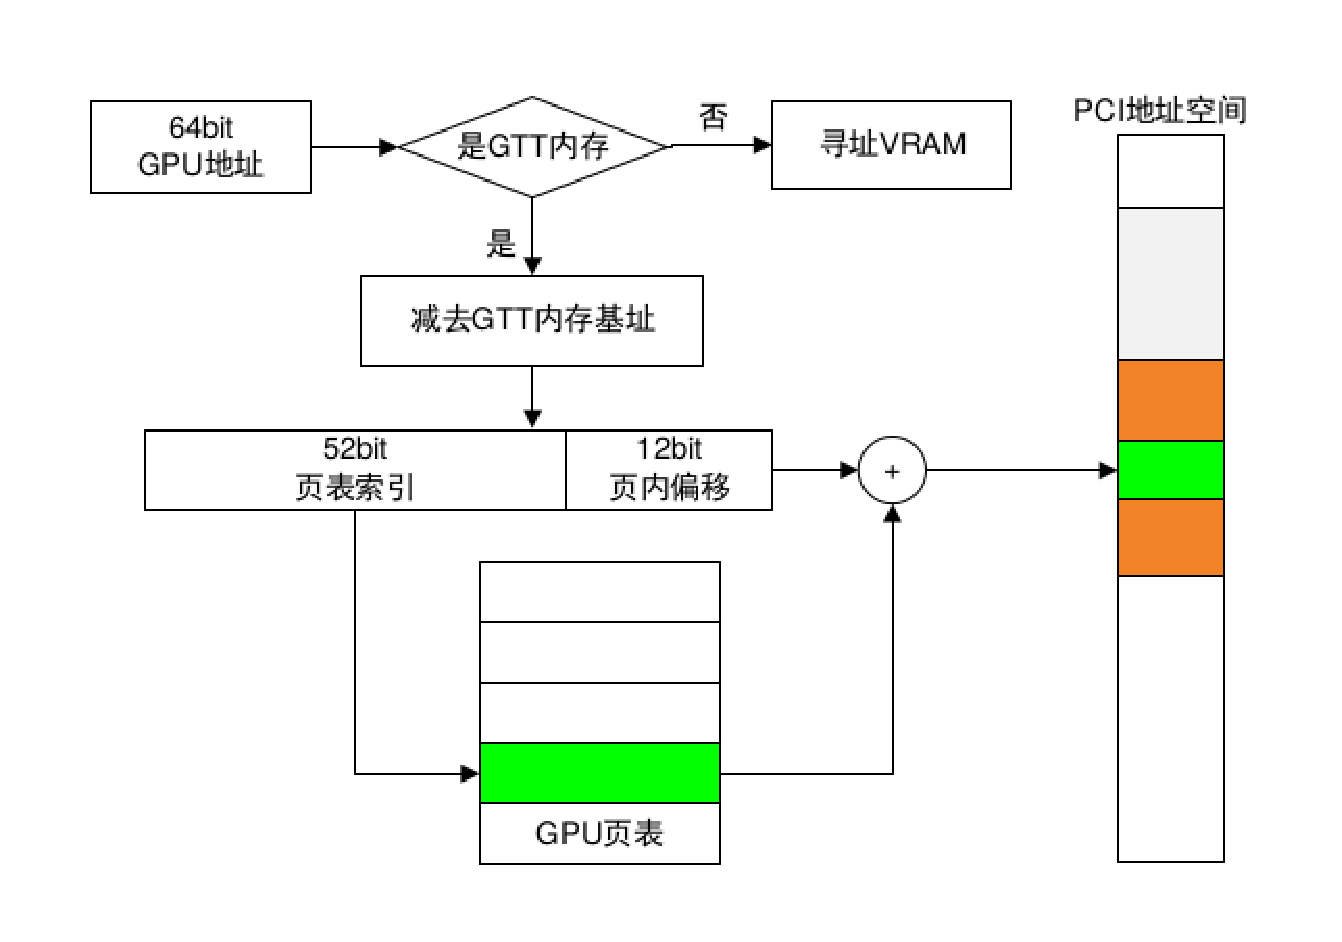
\includegraphics[width=12cm,height=8cm]{figures/chap03/gpu-mmu}
  \caption{GPU的内存访问机制}
  \label{fig:gpu-mmu}
\end{figure}

与此同时,CPU使用的内存就复杂的多了,CPU通过MMU单元将虚拟地址转化成实际的物理地址,这些物理地址有的是系统主存的地址,有些是外接设备的地址,其中就包括GPU的自带显存VRAM地址。通过下图\ref{fig:cpu-gpu-mm}可以看到,CPU和GPU均能自有访问系统内存和显卡内存VRAM。

\begin{figure}[H] 
  \centering
  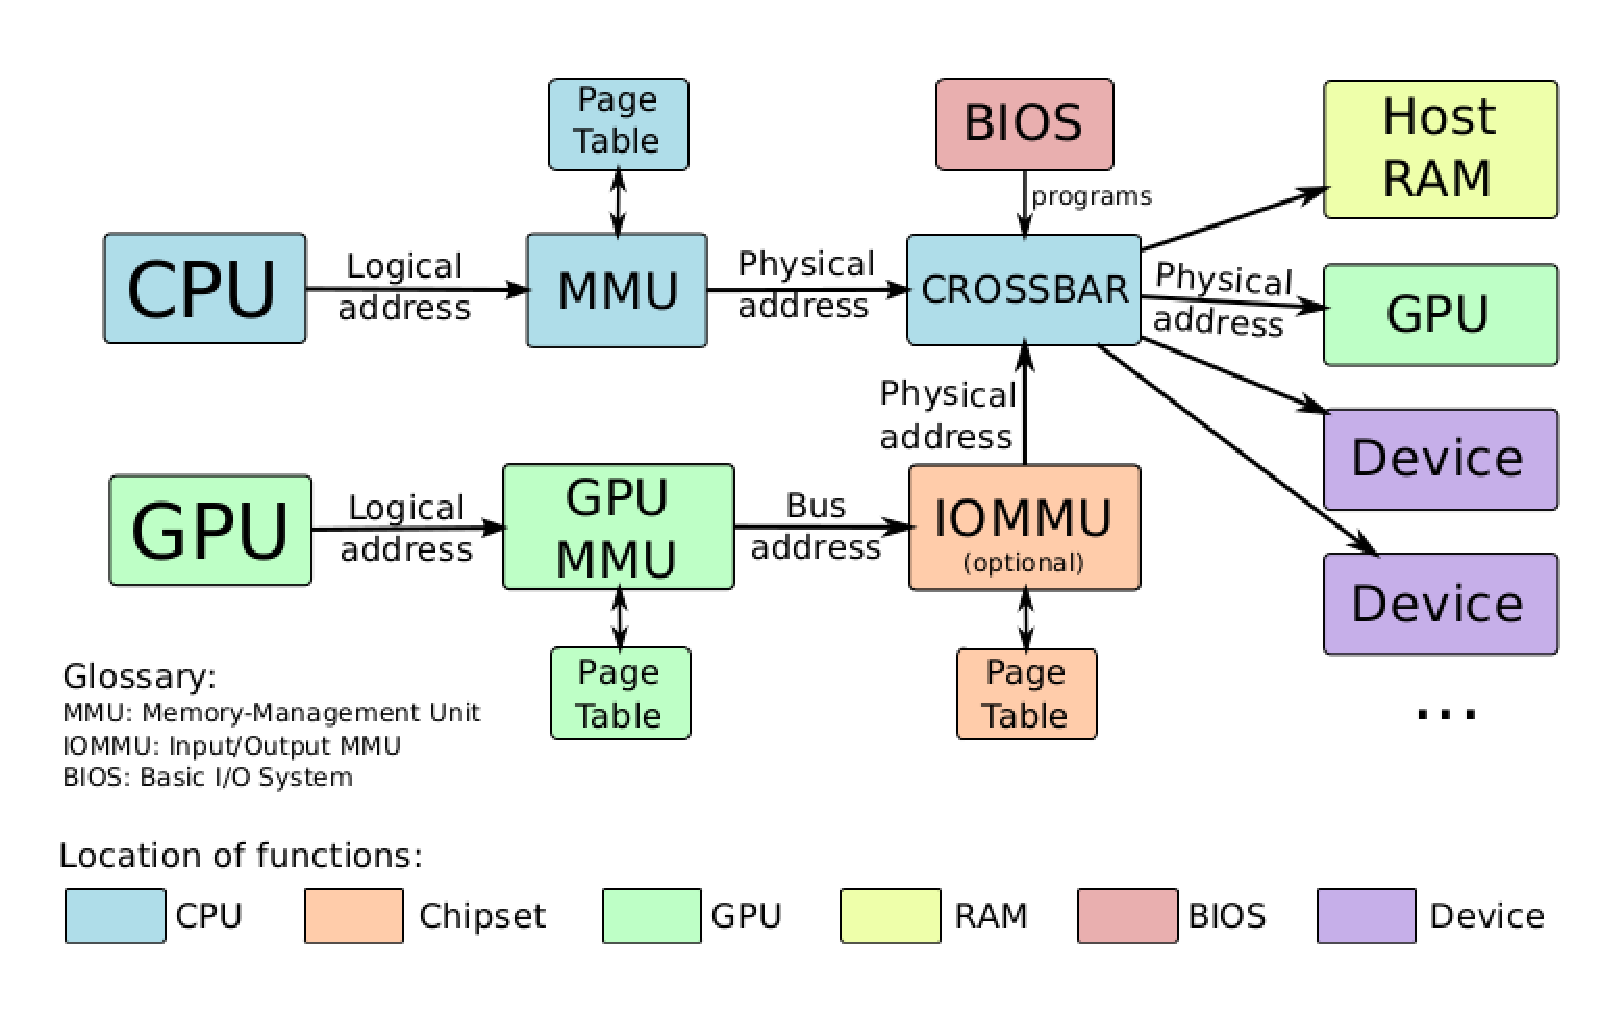
\includegraphics[width=12cm,height=8cm]{figures/chap03/cpu-gpu-mm}
  \caption{CPU与GPU内存请求回路}
  \label{fig:cpu-gpu-mm}
\end{figure}

\subsubsection{龙芯平台下内存与显存传输的性能分析}

从CPU的角度来说我们可以看到存在着两种内存传输: 系统内存到系统内存(cache)、系统内存到显存。这里本文以龙芯3A搭载Radeon R600显卡平台为例测试并研究这两种传输的性能。得到相关数据如下表\ref{tab:memcpy-performance}所示:

\begin{center} \tablecaption{龙芯3A访存性能分析 \label{tab:memcpy-performance}} 
\tablefirsthead{
\rowcolor[gray]{0.8}
\multicolumn{1}{c}{\textbf{数据量大小}} &
\multicolumn{1}{c}{\textbf{内存到内存}} &
\multicolumn{1}{c}{\textbf{内存到显存}} \\ }
\tablehead{\multicolumn{3}{c}{
\small 表 \ref{tab:memcpy-performance} (续) } \\
\rowcolor[gray]{0.8}
\multicolumn{1}{c}{\textbf{数据量大小}} &
\multicolumn{1}{c}{\textbf{内存到内存}} &
\multicolumn{1}{c}{\textbf{内存到显存}} \\ }
\tabletail{\bottomrule
\multicolumn{3}{c}{\small 接下页} \\}
\tablelasttail{\bottomrule}

%./svPerfGL -i ../../trisNormsColors-512.nc -w 1280 -h 1024 -2 -r -t 60 -s 3000000
\begin{supertabular}{p{5.cm}<{\centering}p{5.cm}<{\centering}m{6.cm}<{\centering}}
	4KB& 409MB/s& 12MB/s\\
	16KB& 564MB/s& 14MB/s\\
	64KB& 313MB/s& 14MB/s\\
	256KB& 268MB/s& 14MB/s\\
	1MB& 246MB/s& 14MB/s\\
	4MB& 210MB/s& 14MB/s\\
	16MB& 201MB/s& 14MB/s\\
	64MB& 185MB/s& 14MB/s\\
	256MB& 178MB/s& 14MB/s\\
\end{supertabular}
\end{center}

通过上表\ref{tab:memcpy-performance}我们可以发现龙芯3A平台上内存到显存拷贝效率较低,这里主要是因为内存到显存拷贝数据传输是通过PCI-E总线传输的,而龙芯平台上PCI-E带宽非常的小,所以导致这样直接传输的性能底下。

\subsection{Mesa3D图形库CPU与GPU访存行为分析}

在Mesa3D图形库的实现中,CPU端在初始化过程中会创建顶点对象缓存区,而这些顶点对象缓存区是创建在VRAM之上的,然后通过内存映射的方式映射成CPU端虚拟地址进行访问。在上层程序需要使用Mesa3D进行图形绘制时候,Mesa3D会将绘制相关的顶点数据拷贝到顶点对象缓存区中,即发生了CPU端内存到显存的拷贝,整个过程是同步实现的,即需要占用CPU的指令周期。当GPU接受到绘制命令和相关顶点数据准备好时候,GPU就开始内部的硬件图形加速渲染管线进行图形渲染,并将渲染结果放置到显存的framebuffer中以待显示。以svPerfGL程序顶点数组测试项为例,假如我们需要每帧绘制100万个三角形,那么就会发生三次顶点数据拷贝,分别是顶点位置、顶点颜色和顶点法向量信息,每次拷贝数据量是100万*3*3*4B即36MB数据的大小。

通过上表\ref{tab:memcpy-performance}我们可以看到从内存拷贝到显存这么多数据是非常缓慢的,并且我们通过perf工具测试出整个顶点数组模式测试项的执行时间中百分之九十的时间都花在这个拷贝数据之上,所以成为了程序的性能瓶颈。

\subsection{Mesa3D图形库CPU与GPU访存优化}

针对Mesa3D图形库实际的访存特点,本文从访存策略与拷贝效率这两个方面提出了相应的优化方案。

\subsubsection{CPU与GPU访存策略的优化}
从前面的介绍我们知道,由于CPU端内存到显存的数据拷贝效率低下,导致占用了大量的CPU执行周期,使得CPU执行时间占比过大,而GPU相对执行时间过少。为了改变这一状况,如下图\ref{fig:vbo-gtt}我们可以把顶点数据缓冲区创建在系统内存之上,CPU只需简单的系统内存内部搬运数据,而GPU则通过GTT的方式访问顶点数据缓冲区然后进行图形硬件渲染。

\begin{figure}[H] 
  \centering
  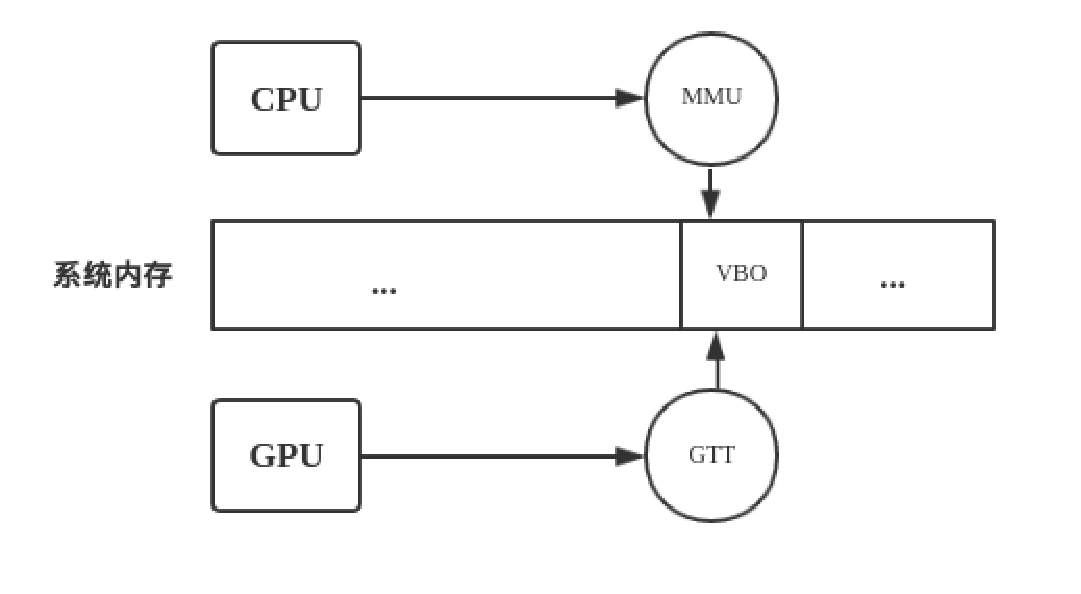
\includegraphics[width=10cm,height=6cm]{figures/chap03/vbo-gtt}
  \caption{Mesa3D图形库CPU与GPU改进后访存策略}
  \label{fig:vbo-gtt}
\end{figure}

虽然这样之后,GPU渲染时候的数据访问效率会降低,但是由于本身GPU工作负担小于CPU,而且因为龙芯平台CPU执行效率相对GPU较弱,所以整个CPU和GPU的并行程度提高了,缩短了整个的执行时间。

\subsubsection{CPU拷贝效率的优化}

在前一节的改进访存策略之后,我们可以通过提高拷贝效率来改进CPU的数据传输性能。由于CPU端向GTT的数据拷贝大多都是单精度浮点数据的拷贝,所以我们可以通过龙芯平台特有的宽位访存指令来提高拷贝效率。

\textbf{龙芯扩展宽位访存指令}: 龙芯平台为了自身发展的需求,通过龙芯指令系统融合技术\cite{loongson-merge},专门开发了一些宽位访存指令,诸如本文使用到的128bit浮点访存指令GSLQ和GSSQ可以实现128bit的浮点数据存取。

由于我们的宽位访存指令GSLQ和GSSQ必须要按照要求先进行128位对齐后使用,所以我们在优化CPU的单精度浮点数据拷贝时候,则必须要考虑到拷贝源地址和目的地址的对齐情况,为了更简明的说明这个问题,我们可以通过下图\ref{fig:memcpy}来看宽位访存指令实现拷贝效率优化的整个过程。

\begin{figure}[H] 
  \centering
  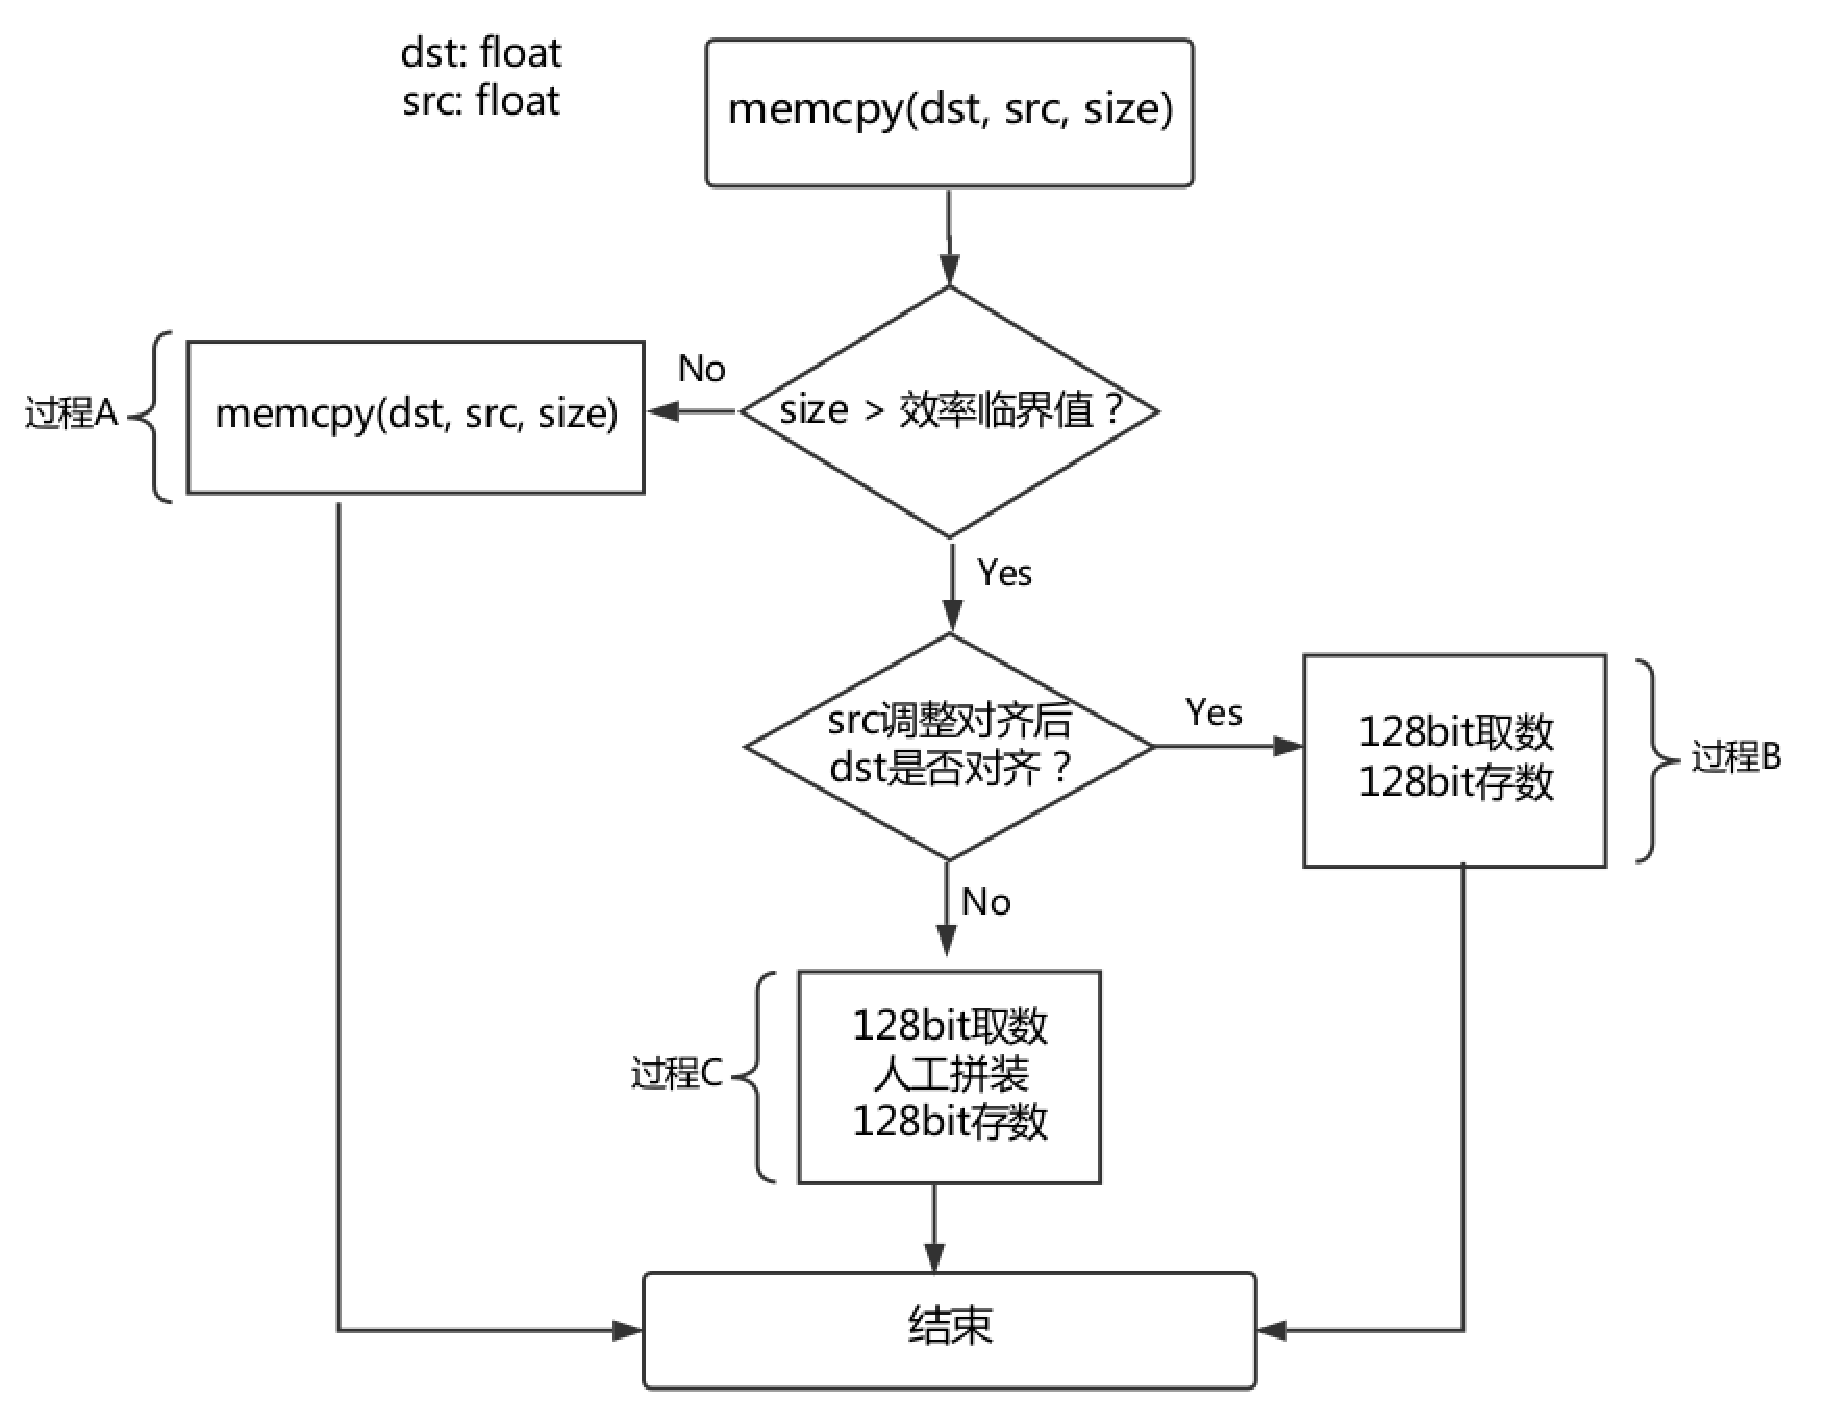
\includegraphics[width=16cm,height=9cm]{figures/chap03/memcpy}
  \caption{宽位访存指令实现拷贝效率优化}
  \label{fig:memcpy}
\end{figure}

这里介绍一下流程图\ref{fig:memcpy}里面的过程A、过程B和过程C的具体工作:

\begin{itemize}

\item{\textbf{过程A}}: 直接调用glibc系统库的memcpy函数。
\item{\textbf{过程B}}: \\
因为这种情况下源地址src和目的地址dst都是128bit对齐的,所以只需要直接的使用宽位访存指令取数和存数即可。相关实现伪代码如下:
\vspace{6pt}
\begin{breakablealgorithm}
	\caption{过程B算法}
	\begin{algorithmic}[1] %每行显示行号
		\Require $dst$目的地址,$src$源地址, $size$大小
		%\Ensure 
		\Function {memcpy}{$dst, src, size$}
			\State $gpr0 \gets src$
			\State $gpr1 \gets dst$
			\State $off \gets 0$
			\While {$off + 16 < size$}
				\State $gslq\, gpr2,\, gpr1,\, off(gpr0)$
				\State $gssq\, gpr2,\, gpr1,\, off(gpr1)$
				\State $off \gets off + 16$
			\EndWhile
		\EndFunction
	\end{algorithmic}
\end{breakablealgorithm}
\vspace{6pt}

\item{\textbf{过程C}}: \\
由于在源地址src对齐后,目的地址dst不是128bit对齐的,所以这里目的地址dst与128bit对齐地址的差可能会是32bit、64bit和96bit这三种,然后无论哪一种都需要我们进行人工的暂存和拼接组装。实现伪代码如下:
\vspace{6pt}
\begin{breakablealgorithm}
	\caption{过程C算法}
	\begin{algorithmic}[1] %每行显示行号
		\Require $dst$目的地址,$src$源地址, $size$大小
		%\Ensure 
		\Function {memcpy}{$dst, src, size$}
			\State $array pre[0:3] \gets \{0.0f, 0.0f, 0.0f, 0.0f\}$
			\State $array cur[0:3] \gets \{0.0f, 0.0f, 0.0f, 0.0f\}$
			\State $offbit \gets (dst \% 16) * 8$
			\State $n \gets offbit/32 - 1$
			\State $pre[0:n] \gets src[0:n]$
			\State $off \gets 16$
			\State $gpr0 \gets src + off$
			\State $gpr1 \gets dst + off - offbit/8$
			\While {$off + 16 < size$}
				\State $gslq\, gpr2, gpr3, off(gpr0)$
				\State $cur[n+1:3]  \gets \{gpr2, gpr3\}\, low\, 128-offbit\, bit$
				\State $cur[0:n] \gets pre[0:n]$
				\State $pre[0:n] \gets \{gpr2, gpr3\}\, high\, offbit\, bit$
				\State ${gpr2, gpr3} \gets cur[0:3]$
				\State $gssq\, gpr2,\, gpr3,\, off(gpr1)$
				\State $off \gets off + 16$
			\EndWhile
		\EndFunction
	\end{algorithmic}
\end{breakablealgorithm}
\vspace{6pt}

\end{itemize}

这里以目的地址dst与128bit对齐地址偏移32bit为例来解释上述过程C算法。如下图\ref{fig:offset32}所示,我们需要将src开始的源数据搬运到dst开始的目的位置,此时src已经是128bit对齐,而dst与128bit对齐相差32bit,这时我们将s4位置的32bit数据暂存起来,接着采用宽位访存指令读取src下一个128bit数据,即\{s5,s6,s7,s8\},接着我们将s4,s5,s6,s7拼装起来成128bit采用宽位访存指令存储到dst的下一个128bit对齐位置,即{d4,d5,d6,d7}。以此规律循环处理即可完成非对齐情况下的数据拷贝。


\begin{figure}[H] 
  \centering
  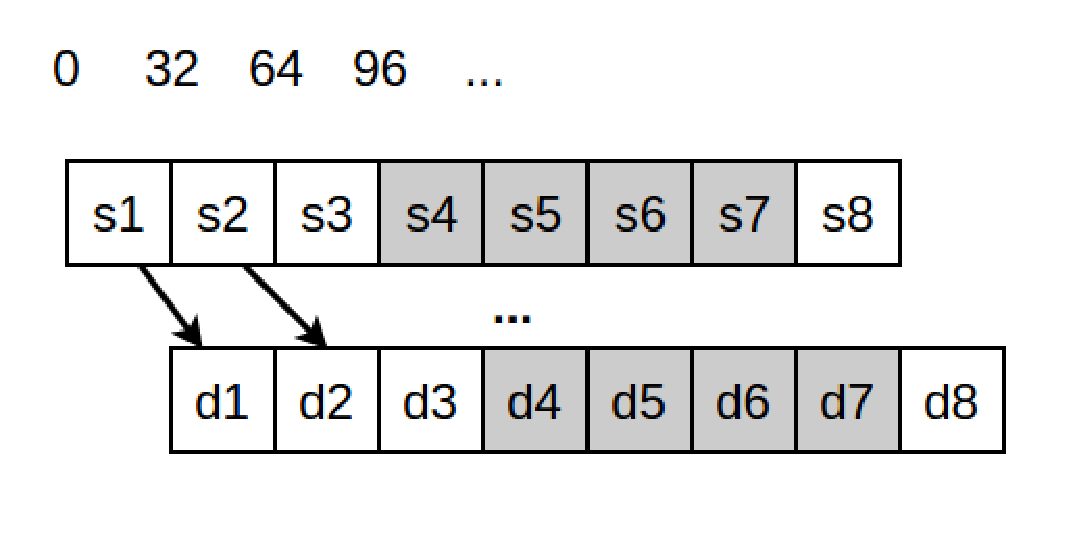
\includegraphics[width=10cm,height=6cm]{figures/chap03/offset32}
  \caption{32bit偏移下过程C算法举例}
  \label{fig:offset32}
\end{figure}

这里为了验证宽位访存指令的效果,进行了内存到内存的拷贝性能测试,测试结果如下:

\begin{center} \tablecaption{宽位访存指令优化效果测试 \label{tab:memcpy-performance-opt}} 
\tablefirsthead{
\rowcolor[gray]{0.8}
\multicolumn{1}{c}{\textbf{数据量大小}} &
\multicolumn{1}{c}{\textbf{优化前}} &
\multicolumn{1}{c}{\textbf{优化后}} \\ }
\tablehead{\multicolumn{3}{c}{
\small 表 \ref{tab:memcpy-performance-opt} (续) } \\
\rowcolor[gray]{0.8}
\multicolumn{1}{c}{\textbf{数据量大小}} &
\multicolumn{1}{c}{\textbf{优化前}} &
\multicolumn{1}{c}{\textbf{优化后}} \\ }
\tabletail{\bottomrule
\multicolumn{3}{c}{\small 接下页} \\}
\tablelasttail{\bottomrule}

%./svPerfGL -i ../../trisNormsColors-512.nc -w 1280 -h 1024 -2 -r -t 60 -s 3000000
\begin{supertabular}{p{6.cm}<{\centering}p{3.cm}<{\centering}m{6.cm}<{\centering}}
	4KB& 409MB/s& 819MB/s\\
	16KB& 564MB/s& 1260MB/s\\
	64KB& 313MB/s& 420MB/s\\
	256KB& 268MB/s& 399MB/s\\
	1MB& 246MB/s& 325MB/s\\
	4MB& 210MB/s& 227MB/s\\
	16MB& 201MB/s& MB/s\\
	64MB& 185MB/s& MB/s\\
	256MB& 178MB/s& 183MB/s\\
\end{supertabular}
\end{center}

\subsubsection{GPU拷贝效率的优化}

前面提到的CPU与GPU拷贝策略的优化是把数据放在GTT,然后让GPU来GTT访问数据,这样可能会加大GPU的负载,所以这里采用张凯的论文$<<$显存与内存间的数据传输通路优化$>>$\cite{gpu-cpu-data}里面提到采用GTT+DMA的这种非线性的优化方法,使用这种方法的原理就是GPU采用DMA的方式在不占用CPU的执行周期的情况下将GTT里面的内容快速的拷贝到显存中,这样GPU之后的访存时间就会减少,总体上减小了GPU的工作负载。

\begin{figure}[H] 
  \centering
  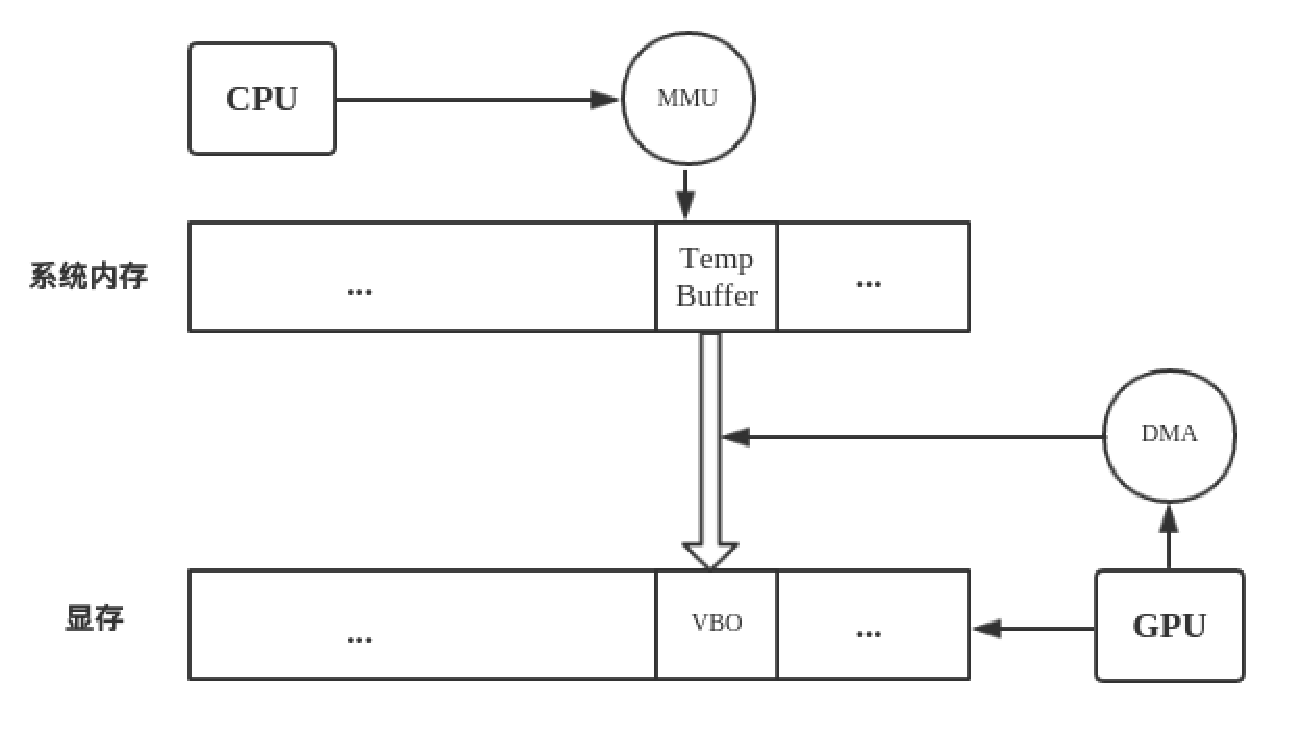
\includegraphics[width=12cm,height=8cm]{figures/chap03/gpu-dma}
  \caption{DMA方式下的Mesa3D库CPU与GPU访存策略}
  \label{fig:gpu-dma}
\end{figure}

改进的传输模式如图\ref{fig:gpu-dma},对比之前的实现(图\ref{fig:vbo-gtt}),虽然设计上更加复杂了一些,但是在龙芯平台上,PCI-E总线带宽较小,直接读写的速度非常慢, 这会导致即使在小数据量时直接读写的效率也比DMA方式的效率更低。
